%%%%%%%%%%%%%%%%%%%%%%%%%%%%%%%%%%%%%%%%%
% Beamer Presentation
% LaTeX Template
% Version 1.0 (10/11/12)
%
% This template has been downloaded from:
% http://www.LaTeXTemplates.com
%
% License:
% CC BY-NC-SA 3.0 (http://creativecommons.org/licenses/by-nc-sa/3.0/)
%
%%%%%%%%%%%%%%%%%%%%%%%%%%%%%%%%%%%%%%%%%

%----------------------------------------------------------------------------------------
%	PACKAGES AND THEMES
%----------------------------------------------------------------------------------------

\documentclass{beamer}

\mode<presentation> {

% The Beamer class comes with a number of default slide themes
% which change the colors and layouts of slides. Below this is a list
% of all the themes, uncomment each in turn to see what they look like.

%\usetheme{default}
%\usetheme{AnnArbor}
%\usetheme{Antibes}
%\usetheme{Bergen}
%\usetheme{Berkeley}
%\usetheme{Berlin}
%\usetheme{Boadilla}
%\usetheme{CambridgeUS}
%\usetheme{Copenhagen}
%\usetheme{Darmstadt}
%\usetheme{Dresden}
\usetheme{Frankfurt}
%\usetheme{Goettingen}
%\usetheme{Hannover}
%\usetheme{Ilmenau}
%\usetheme{JuanLesPins}
%\usetheme{Luebeck}
%\usetheme{Madrid}
%\usetheme{Malmoe}
%\usetheme{Marburg}
%\usetheme{Montpellier}
%\usetheme{PaloAlto}
%\usetheme{Pittsburgh}
%\usetheme{Rochester}
%\usetheme{Singapore}
%\usetheme{Szeged}
%\usetheme{Warsaw}

% As well as themes, the Beamer class has a number of color themes
% for any slide theme. Uncomment each of these in turn to see how it
% changes the colors of your current slide theme.

%\usecolortheme{albatross}
%\usecolortheme{beaver}
%\usecolortheme{beetle}
%\usecolortheme{crane}
%\usecolortheme{dolphin}
%\usecolortheme{dove}
%\usecolortheme{fly}
%\usecolortheme{lily}
%\usecolortheme{orchid}
%\usecolortheme{rose}
%\usecolortheme{seagull}
%\usecolortheme{seahorse}
%\usecolortheme{whale}
%\usecolortheme{wolverine}

%\setbeamertemplate{footline} % To remove the footer line in all slides uncomment this line
%\setbeamertemplate{footline}[page number] % To replace the footer line in all slides with a simple slide count uncomment this line

%\setbeamertemplate{navigation symbols}{} % To remove the navigation symbols from the bottom of all slides uncomment this line
}

\usepackage{graphicx} % Allows including images
\usepackage{booktabs} % Allows the use of \toprule, \midrule and \bottomrule in tables
\usepackage[brazilian]{babel}
\usepackage[utf8]{inputenc}
\usepackage[T1]{fontenc}
\usepackage{amsmath}
\usepackage{animate}

%----------------------------------------------------------------------------------------
%	TITLE PAGE
%----------------------------------------------------------------------------------------

\title[PSO]{Particle Swarm Optimization} % The short title appears at the bottom of every slide, the full title is only on the title page

\author{Bruno Iochins Grisci} % Your name
\institute[UFRGS] % Your institution as it will appear on the bottom of every slide, may be shorthand to save space
{
Universidade Federal do Rio Grande do Sul \\ % Your institution for the title page
\medskip
\textit{bigrisci@inf.ufrgs.br} % Your email address
}
\date{\today} % Date, can be changed to a custom date

\begin{document}

\begin{frame}
\titlepage % Print the title page as the first slide
\end{frame}

\begin{frame}
\frametitle{Sumário} % Table of contents slide, comment this block out to remove it
\tableofcontents % Throughout your presentation, if you choose to use \section{} and \subsection{} commands, these will automatically be printed on this slide as an overview of your presentation
\end{frame}

%----------------------------------------------------------------------------------------
%	PRESENTATION SLIDES
%----------------------------------------------------------------------------------------

%------------------------------------------------
\section{Inspiração} % Sections can be created in order to organize your presentation into discrete blocks, all sections and subsections are automatically printed in the table of contents as an overview of the talk
%------------------------------------------------

\begin{frame}
\frametitle{Inspiração}
Técnica de otimização inspirada no comportamento de grupos de animais como cardumes de peixes ou enxames de insetos.
\begin{figure}[htbp]
  \begin{minipage}[b]{0.4\linewidth}
    \centering
    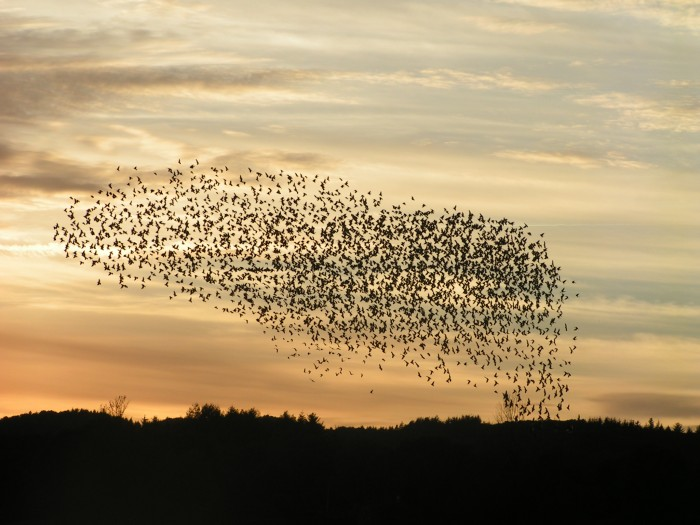
\includegraphics[width=\linewidth]{birds.jpg}
  \end{minipage}
  \hspace{0.5cm}
  \begin{minipage}[b]{0.4\linewidth}
    \centering
    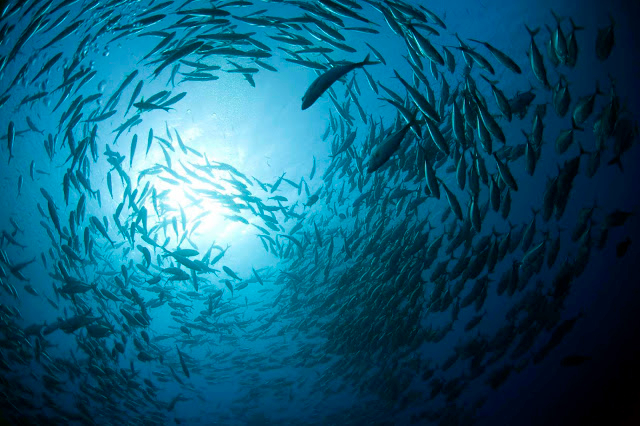
\includegraphics[width=\linewidth]{fish.jpg}
  \end{minipage}
\end{figure}
\end{frame}

%------------------------------------------------
\section{Características} 
%------------------------------------------------

\begin{frame}
\frametitle{Características}
\begin{itemize}
\item Criado na década de 1990;
\item Método baseado em populações estáticas (enxame de partículas);
\item Sem qualquer tipo de seleção;
\item Utiliza mutação dirigida;
\item Opera com métricas multidimensionais;
\item Normalmente com valores reais;
\item Partículas são mutadas em direção à melhor solução conhecida.
\end{itemize}
\end{frame}

\begin{frame}
 \frametitle{Exemplo}
 \animategraphics[loop,controls,width=0.9\linewidth]{12}{ParticleSwarmArrowsAnimation-}{0}{99}
\end{frame}


%------------------------------------------------
\section{Pseudocódigo}
%------------------------------------------------

\begin{frame}
\frametitle{Pseudocódigo}
\begin{figure}
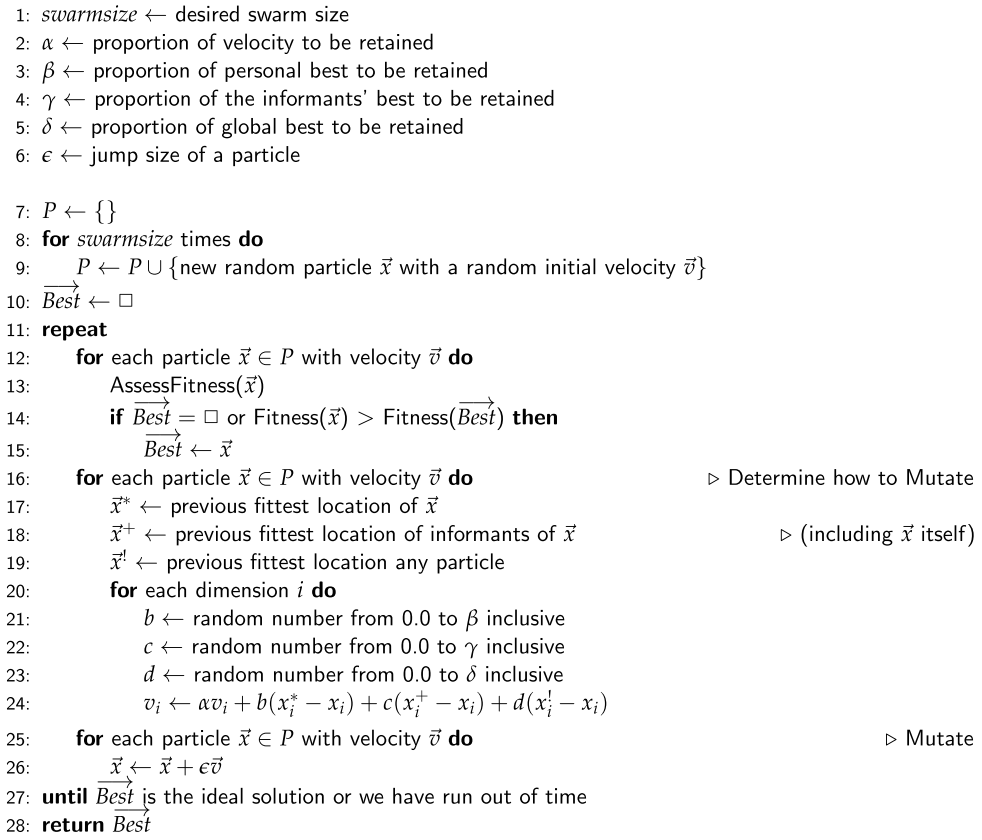
\includegraphics[width=0.65\linewidth]{psocode.png}
\end{figure}
\footnotesize{
Retirado de Essentials of Metaheuristics (Sean Luke, 2015).
}
\end{frame}

%------------------------------------------------
\section{Aplicações}
%------------------------------------------------

\begin{frame}
\frametitle{Aplicações}
Usos de PSO incluem:
\begin{itemize}
\item Treinamento de redes neurais;
\item Telecomunicações;
\item Sistemas de energia;
\item Otimização combinatorial;
\item Processamento de sinais;
\end{itemize}
A metaheurística é usada principalmente em problemas de otimização unimodais sem restrições, mas também foi demonstrada sua utilidade em problemas multi-objetivo, multimodais, com restrições e com variação dinâmica. 
\end{frame}

%------------------------------------------------
\section{Implementação}
%------------------------------------------------

\begin{frame}
\frametitle{Implementação}
\begin{itemize}
\item Python;
\item Nunpy;
\item Orientado a Objetos:
\begin{itemize}
\item Modularidade;
\item Reúso;
\item Versatilidade
\end{itemize}
\end{itemize}
\end{frame}

\begin{frame}
\frametitle{Representação}
Para n átomos:

location = [x, y, z, x, y, z]

velocity = [x, y, z, x, y, z]

locations = M[n][6]

velocities = M[n][6]
\end{frame}

\begin{frame}
\frametitle{Controle dos limites}
Novas velocidades podem gerar soluções fora do espaço de busca permitido.
\begin{figure}
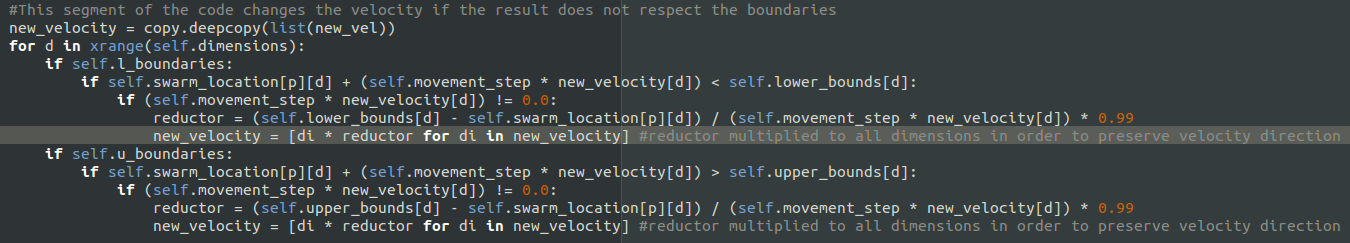
\includegraphics[width=1.0\linewidth]{pylimit.png}
\end{figure}
\end{frame}

\begin{frame}
\frametitle{Controle do laço}
\begin{figure}
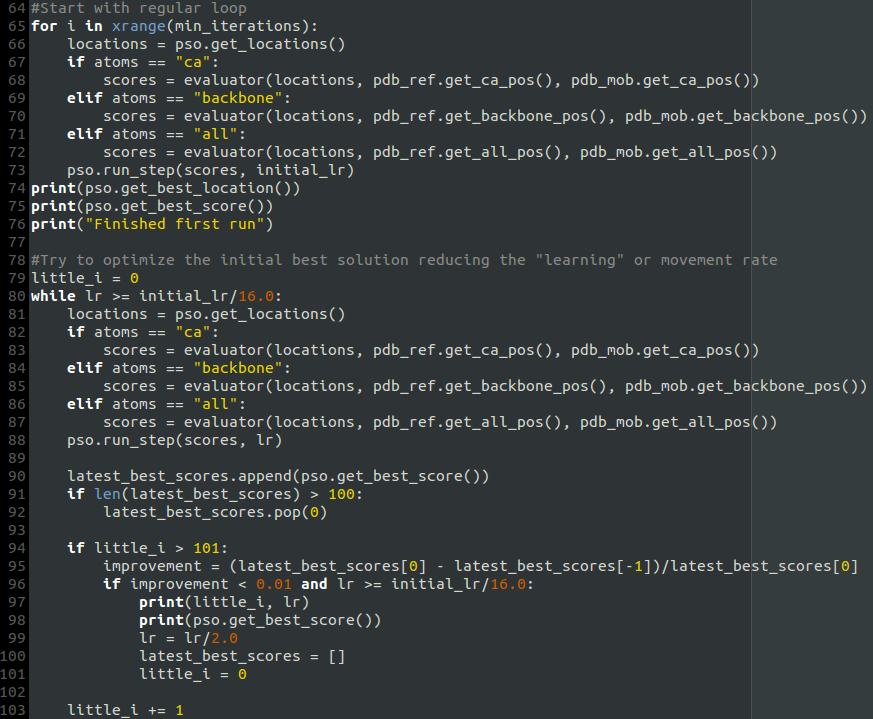
\includegraphics[width=0.8\linewidth]{pyloop.png}
\end{figure}
\end{frame}

\begin{frame}
\frametitle{Leitura do .pdb}
Recupera:
\begin{itemize}
\item Nome dos átomos;
\item Índice dos resíduos de aminoácidos;
\item Coordenadas cartesianas dos átomos;
\end{itemize}
Alinha os átomos de dois arquivos .pdb.
\end{frame}

\begin{frame}
\frametitle{Translação e rotação}
\begin{figure}
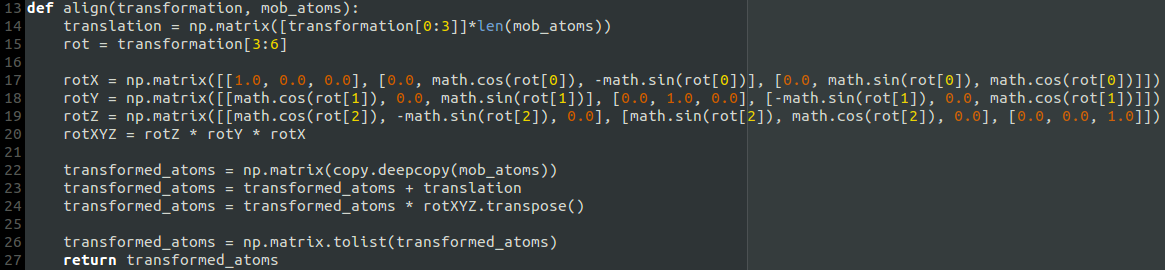
\includegraphics[width=1.0\linewidth]{pyrot.png}
\end{figure}
\end{frame}

%------------------------------------------------
\section{Resultados}
%------------------------------------------------

\begin{frame}
\frametitle{Resultados}
\begin{table}[]
\centering
\label{my-label}
\begin{tabular}{lllll}
          & BACKBONE          & CA            & ALL    & PYMOL           \\
REFERENCE & 0.0002 & 5.84E-007     & 0.0002 & 0.000 \\
1ACW-01   & 13.5292     & 13.5886 & 14.5882 & 13.570   \\
1ACW-02   & 14.1559     & 14.2188 & 14.8492 & 14.216    \\
1ACW-03   & 11.5880     & 11.7586 & 12.4787 & 11.758   \\
1ACW-04   & 12.3860     & 12.3765 & 13.1628 & 6.827  \\
1ACW-05   & 12.6750     & 12.7391 & 13.6928 & 11.730   \\
1ACW-06   & 15.6788     & 15.7296 & 16.2010 & 15.729                   
\end{tabular}
\end{table}
\end{frame}

%------------------------------------------------
\section{Referências}
%------------------------------------------------

\begin{frame}
\frametitle{Referências}
\footnotesize{
\begin{thebibliography}{99} % Beamer does not support BibTeX so references must be inserted manually as below
\bibitem[Luke, 2015]{p1} Sean Luke (2015)
\newblock Essentials of Metaheuristics

\bibitem[Padhye, 2012]{p1} Nikhil Padhye (2012)
\newblock Boundary Handling Approaches in Particle Swarm Optimization
\newblock \emph{KanGAL Report Number 2012014}.

\end{thebibliography}
}
\end{frame}

%------------------------------------------------

\begin{frame}
\Huge{\centerline{Fim}}
\end{frame}

%----------------------------------------------------------------------------------------

\end{document} 